\chapter{Physically-Inspired Excitations}\label{ch:physInspExcitations}
This short chapter introduces several simple ways to excite the different resonators presented in Part \ref{part:resonators}. First, various ways to excite resonators using initial conditions are provided, after which examples of time-varying excitations are given, such that the systems can also be excited later during the simulation.

\section{Initial conditions}\label{sec:initConditionsPhysInsp}
The easiest way to excite a system is to set its initial conditions to non-zero values. This has been done several times before using a raised cosine (see e.g. Section \ref{sec:output1DWave}). To give the system an initial displacement, not an initial velocity, one initialises both $u^0_l$ and $u^1_l$ with the same values. In the following, the 1D wave equation will be used as an example (Eq. \eqref{eq:1DwavePDE}):
\begin{equation}
    \ptt u = c^2 \pxx u
\end{equation}
where $u=u(x,t)$ is the state of the system defined for $t\geq 0$ and $x\in D$ with domain $\D = [0, L]$ and length $L$ (in m). Furthermore, $c = 735$ m/s. Following \ref{sec:gridFunctions}, the state variable can be discretised to $\uln$ where $n\in \mathbb{N}^0$ and $l\in d$ with discrete domain $d = \{0, \hdots, N\}$ and number of grid points $N+1$. The FD scheme is (Eq. \eqref{eq:1DwaveFDS})
\begin{equation}
    \dtt \uln = c^2 \dxx \uln.
\end{equation}

\subsection{Impulse}
The simplest way to excite a system is to set the value of one grid point to non-zero, which is referred to as an \textit{impulse} excitation. Figure \ref{fig:impulse} shows an implementation of the 1D wave equation where $u_l^0 = u_l^1 = 1$ at $l = \floor[0.5 N]$. One can observe that the variations between two neighbouring grid points are extremely high. If the CFL condition in Eq. \eqref{eq:CFL} is satisfied with equality, the system will exhibit high amounts of energy around the Nyquist frequency, which is generally unwanted.

\def\figWidth{0.32}
\begin{figure}[h]
    \centering
    \subfloat[$n = 1$.\label{fig:impulse1}]{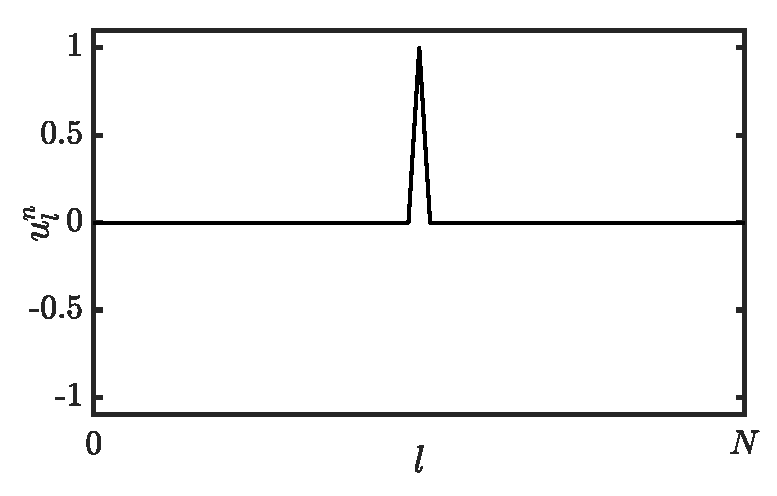
\includegraphics[width=\figWidth\textwidth]{figures/exciters/physInsp/impulse1.eps}}\hfill
    \subfloat[$n = 6$.\label{fig:impulse2}]{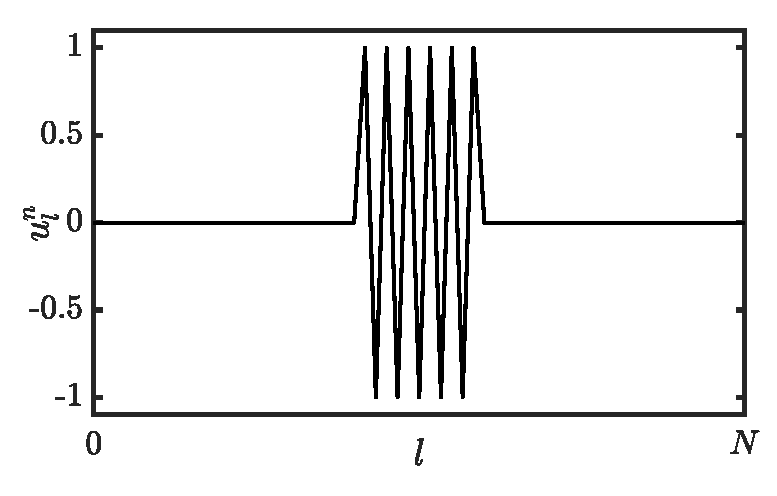
\includegraphics[width=\figWidth\textwidth]{figures/exciters/physInsp/impulse2.eps}}\hfill
    \subfloat[$n = 11$.\label{fig:impulse3}]{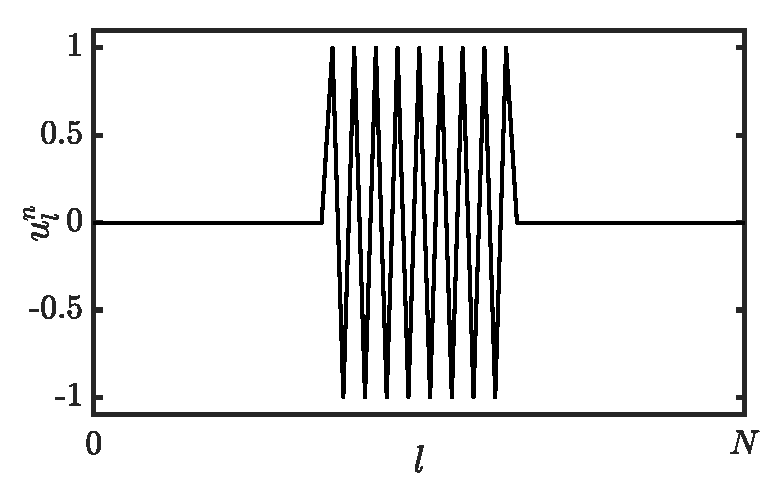
\includegraphics[width=\figWidth\textwidth]{figures/exciters/physInsp/impulse3.eps}}
    \caption{The 1D wave equation initialised with an impulse at $l=\floor[0.5N]$.\label{fig:impulse}}
\end{figure}

\subsection{Raised cosine}\label{sec:raisedCosine}
To avoid the high-frequency behaviour caused by the impulse, a spatially smooth excitation must be created. The \textit{raised cosine} is most often used for this property and is extensively used throughout the literature \cite{theBible}. Initialising the displacement of a distributed system with a raised cosine can be interpreted as a pluck. A different pluck excitation is presented in Section \ref{sec:pluck}.

A raised cosine is parametrised by its amplitude $e_\text{amp}$, its center location $x_0$ and its width $x_\text{w}$. Applied to a distributed 1D system defined over domain $x\in \D$, the (continuous-time) excitation function containing a raised cosine is defined as 
\begin{equation}\label{eq:raisedCosCont}
    e_\text{rc}(x) = 
    \begin{cases}
        \frac{e_\text{amp}}{2}\left(1 - \cos\left(\frac{2\pi (x - x_\stxt)}{x_\text{w}}\right)\right), & \text{if } x_\stxt \leq x \leq x_\etxt,\\
        0, & \text{otherwise},
    \end{cases}
\end{equation}
where 
\begin{equation}\label{eq:xsxe}
    x_\stxt = x_0 - 
    \frac{x_\text{w}}{2}, \qaq x_\etxt = x_0 + \frac{x_\text{w}}{2}
\end{equation}
are the start and end locations of the excitation. Furthermore, $x_\stxt, x_\etxt \in \D$, which puts a constraint on the width and location of the excitation. 

In discrete time\footnote{One could sample the continuous function in Eq. \eqref{eq:raisedCosCont} at locations $x=lh$. In this chapter, looking towards straightforward implementation, a more practical approach has been chosen, and discrete definitions are given separately.}, the center location is defined as $l_0 = \floor[x_0 / h]$, where $\floor[\cdot]$ denotes the flooring operation, $h$ is the grid spacing. The discrete start and end locations of the raised cosine are
\begin{equation}\label{eq:lsle}
    l_\text{s} = l_0 - \floor[w/2]\qaq l_\etxt = l_0 + \floor[w/2],
\end{equation}
with $l_\stxt, l_\etxt\in d$ and, finally, $w = \floor[x_\text{w} / h]$.\footnote{Notice that the width is given in `number of grid spacings' and will thus affect $w+1$ grid points. This is also why the range in Eq. \eqref{eq:raisedCosDisc} includes both end points.} Equation \eqref{eq:raisedCosCont} can then be discretised as
\begin{equation}\label{eq:raisedCosDisc}
    E_{l, \text{rc}} =
    \begin{cases}
        \frac{e_\text{amp}}{2}\left(1 - \cos\left(\frac{2\pi (l - l_\stxt)}{w}\right)\right), & \text{if } l_\stxt \leq l \leq l_\etxt,\\
        0, & \text{otherwise}.
    \end{cases}
\end{equation}
Figure \ref{fig:raisedCos} shows the 1D wave equation initialised with a raised cosine with $e_\text{amp} = 1$, $l_0 = \floor[0.5N]$ and $w = \floor[0.1N]$. Notice that the behaviour is much more smooth than the impulse shown in Figure \ref{fig:impulse}.

\def\figWidth{0.32}
\begin{figure}[h]
    \centering
    \subfloat[$n = 1$.\label{fig:raisedCos1}]{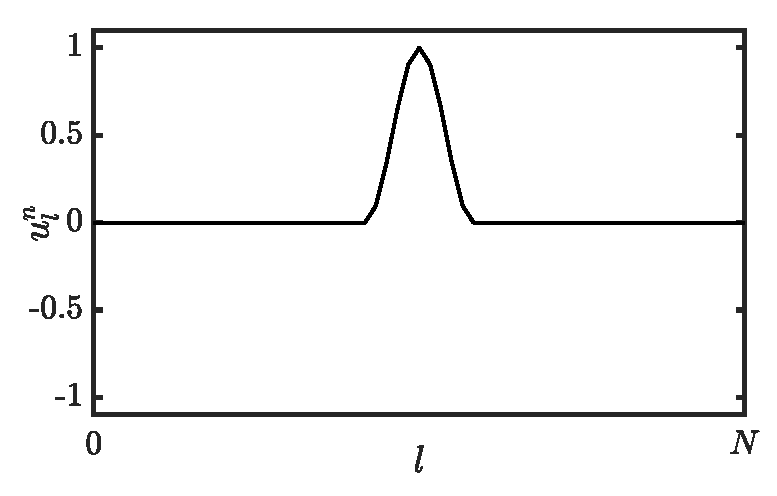
\includegraphics[width=\figWidth\textwidth]{figures/exciters/physInsp/raisedCos1.eps}}\hfill
    \subfloat[$n = 6$.\label{fig:raisedCos2}]{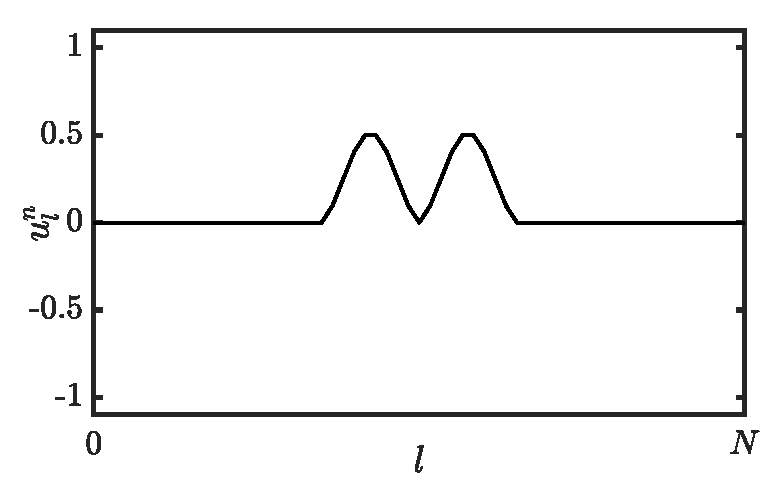
\includegraphics[width=\figWidth\textwidth]{figures/exciters/physInsp/raisedCos2.eps}}\hfill
    \subfloat[$n = 11$.\label{fig:raisedCos3}]{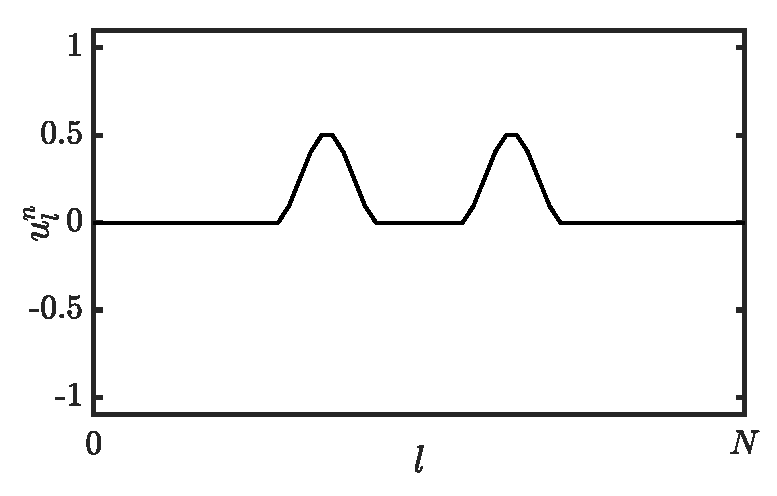
\includegraphics[width=\figWidth\textwidth]{figures/exciters/physInsp/raisedCos3.eps}}
    \caption{The 1D wave equation initialised with a raised cosine at the center of the system.\label{fig:raisedCos}}
\end{figure}

\subsubsection{Strike}\label{sec:strike}
If one initialises the system with an initial velocity, i.e., only setting a displacement at $n=1$, and leaving $u^0_l = 0$ for $l\in d$, one can use the raised cosine to model a strike. Figure \ref{fig:strike} shows a strike using the same values as for the pluck in Figure \ref{fig:raisedCos} at $n=1$, but leaving $u_l^0 = 0$. One can observe that, for the pluck, the displacement of the system stays high rather than going back to 0 as in the case of the pluck. Furthermore, the amplitude of the displacement is higher than for the pluck (notice the scaling of the y-axis).%\footnote{In the case of the 1D wave equation struck using a raised cosine, the maximum amplitude can be calculated to be half of the summed values of the excitation.}

\def\figWidth{0.32}
\begin{figure}[h]
    \centering
    \subfloat[$n = 1$.\label{fig:strike1}]{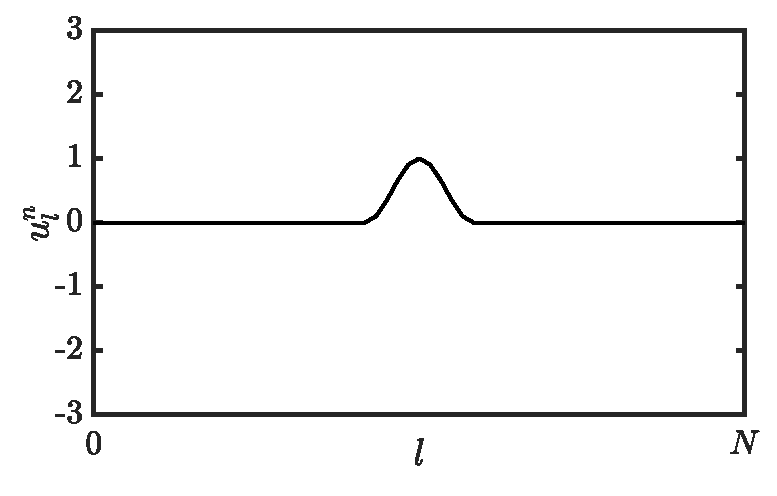
\includegraphics[width=\figWidth\textwidth]{figures/exciters/physInsp/strike1.eps}}\hfill
    \subfloat[$n = 6$.\label{fig:strike2}]{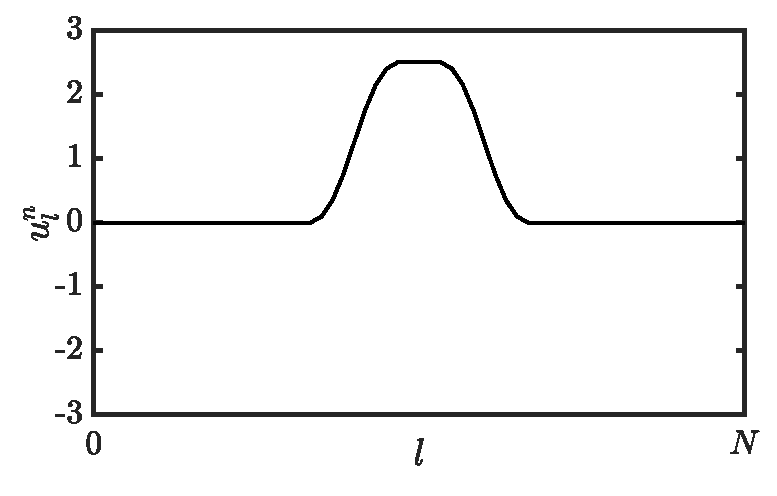
\includegraphics[width=\figWidth\textwidth]{figures/exciters/physInsp/strike2.eps}}\hfill
    \subfloat[$n = 11$.\label{fig:strike3}]{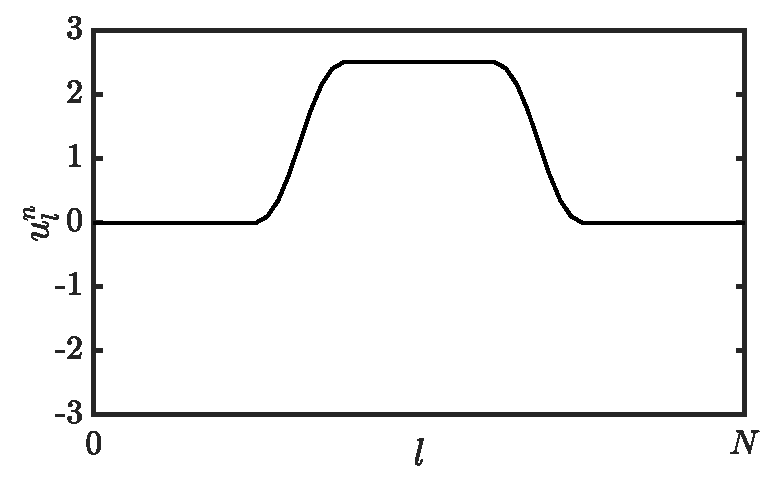
\includegraphics[width=\figWidth\textwidth]{figures/exciters/physInsp/strike3.eps}}
    \caption{The 1D wave equation initialised with a strike at the center of the system. Notice the scaling of the y-axis compared to Figure \ref{fig:raisedCos}. \label{fig:strike}}
\end{figure}

\subsection{Triangular pluck}\label{sec:pluck}
Another way to initialise the string, which is closer to reality, is to use a triangular shape to model a pluck \cite{Fletcher1998, theBible}.%, where the authors analytically decompose the system into its modes of vibration as well as their respective amplitudes depending on the plucking position. 
%
Using $e_\text{amp}$ as the maximum displacement -- at the corner of the triangle -- and $x_0\in \D$ as the plucking position, the triangular excitation can be defined as
\begin{equation}\label{eq:triangleCont}
    e_\text{tri}(x) = \begin{cases}
        \frac{e_\text{amp}}{x_0} x, & \text{if } 0\leq x \leq x_0,\\
        \frac{e_\text{amp}}{x_0 - L} (x - L), &\text{if } x_0 < x \leq L.
    \end{cases}
\end{equation}

In discrete time, Eq. \eqref{eq:triangleCont} becomes 
\begin{equation}
    E_{l, \text{tri}} = \begin{cases}
        \frac{e_\text{amp}}{l_0} l, & \text{if } 0\leq l \leq l_0,\\
        \frac{e_\text{amp}}{l_0 - N} (l - N), &\text{if } l_0 < l \leq N.
    \end{cases}
\end{equation}
Due to the spatial discontinuity at the corner, some high-frequency oscillations (similar to the impulse) might emerge. Figure \ref{fig:pluck} shows an implementation of the 1D wave equation initialised with a triangular pluck excitation. The sample rate is 441 kHz (10x the usual) to prevent these high-frequency oscillations from appearing in the plot (though they still exist to some degree). 

\def\figWidth{0.32}
\begin{figure}[h]
    \centering
    \subfloat[$n = 1$.\label{fig:pluck1}]{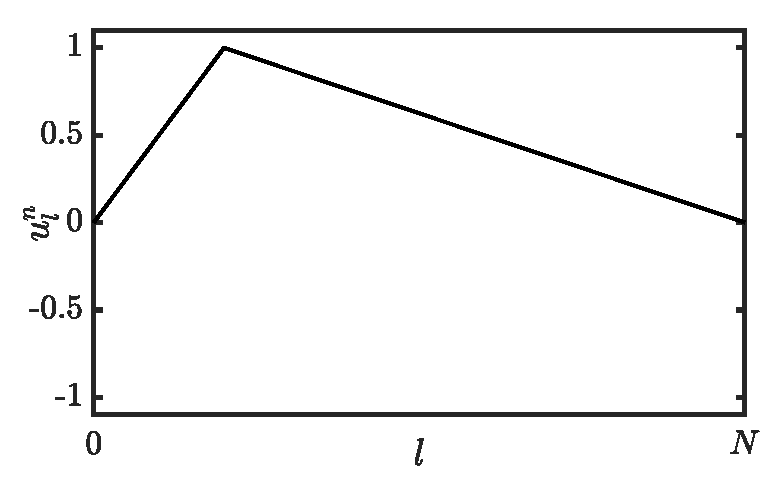
\includegraphics[width=\figWidth\textwidth]{figures/exciters/physInsp/triangle1.eps}}\hfill
    \subfloat[$n = 101$.\label{fig:pluck2}]{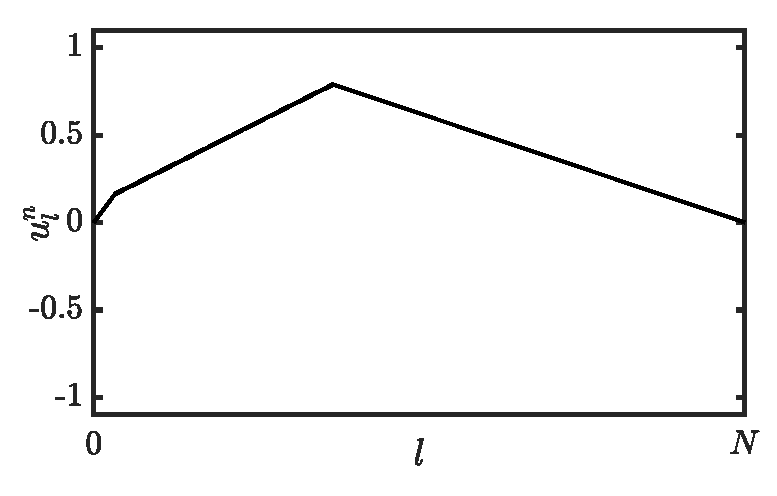
\includegraphics[width=\figWidth\textwidth]{figures/exciters/physInsp/triangle2.eps}}\hfill
    \subfloat[$n = 201$.\label{fig:pluck3}]{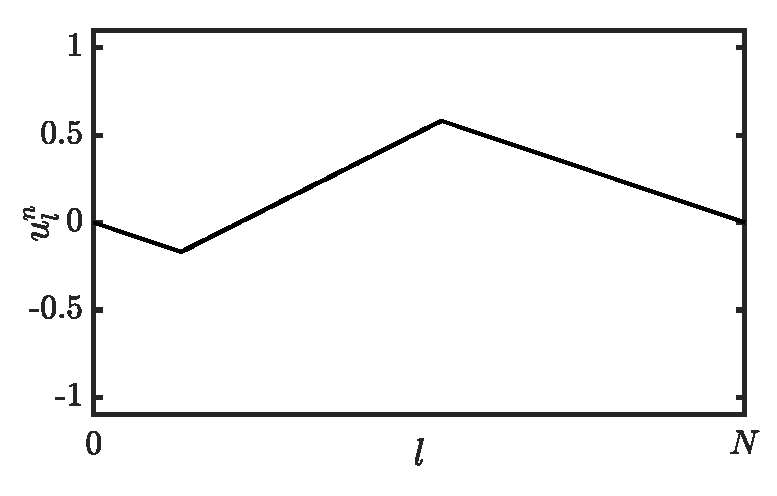
\includegraphics[width=\figWidth\textwidth]{figures/exciters/physInsp/triangle3.eps}}
    \caption{The 1D wave equation initialised with a triangular pluck with $l_0=\floor[0.2N]$. Note that sample rate has been set to $\fs = 441000$ Hz to show a more ideal triangular motion. \label{fig:pluck}}
\end{figure}

\subsection{2D raised cosine}\label{sec:2DraisedCos}
Introducing an extra coordinate $y$, one can extend the raised cosine presented in Section \ref{sec:raisedCosine} to 2D according to 
\begin{equation}\label{eq:raisedCosCont2D}
    e_\text{rc}(x,y)\! =\! 
    \begin{cases}
        \!\frac{e_\text{amp}}{2}\left(1 - \cos\left(\frac{2\pi (x - x_\stxt)}{r_\text{w}}\right)\right)\left(1 - \cos\left(\frac{2\pi (y - y_\stxt)}{r_\text{w}}\right)\right), & 
        \!\!\!\begin{aligned}
            &\text{if } x_\stxt \leq x \leq x_\etxt, \\
            &\text{and } y_\stxt \leq y \leq y_\etxt,
        \end{aligned}\\[1.25em]
        \!0, &\!\! \text{otherwise},
    \end{cases}
\end{equation}
where $r_\text{w}$ is the excitation radius. Similar to Eq. \eqref{eq:xsxe}, the start and end locations of the raised cosine in the $x$ and $y$ direction can be calculated as
\begin{equation*}
    x_\stxt = x_0 - 
    \frac{r_\text{w}}{2}, \quad x_\etxt = x_0 + \frac{r_\text{w}}{2}, \quad y_\stxt = y_0 - 
    \frac{r_\text{w}}{2}, \qaq y_\etxt = y_0 + \frac{r_\text{w}}{2},
\end{equation*}
where $(x_0, y_0)$ is the center coordinate and $x_\stxt, x_\etxt, y_\stxt,  y_\text{e}\in \D$ for a 2D domain $\D$.

In discrete time, Eq. \eqref{eq:raisedCosCont2D} becomes
\begin{equation}\label{eq:2DdiscRaisedCos}
    E_{(l,m), \text{rc}} = 
    \begin{cases}
        \!\frac{e_\text{amp}}{2}\left(1 - \cos\left(\frac{2\pi (l \!-\! l_\stxt)}{r}\right)\right)\!\left(1\! -\! \cos\left(\frac{2\pi (m - m_\stxt)}{r}\right)\right)\!, & \!\!\!\!
        \begin{aligned}
            &\text{if } l_\stxt \leq l \leq l_\etxt, \text{ and}\\
            & m_\stxt \leq m \leq m_\etxt,
        \end{aligned}\\
        \!0, &\!\!\!\! \text{otherwise},
    \end{cases}
\end{equation}
where $r = \floor[r_\text{w} / h]$ is the discrete excitation radius (in `number of grid spacings'). Furthermore, similar to Eq. \eqref{eq:lsle},
\begin{equation}
    l_\text{s} = l_0 - \floor[r/2],\ l_\etxt = l_0 + \floor[r/2],\ m_\text{s} = m_0 - \floor[r/2], \ \text{and} \ m_\etxt = m_0 + \floor[r/2]
\end{equation}
for discrete center coordinate $(l_0, m_0)$ and $l_\stxt, l_\etxt, m_\stxt,  m_\text{e}\in d$ for a discrete 2D domain $d$. 
As in the 1D case, this excitation can be used to model a simple `pluck' and strike for a 2D system. See Figure \ref{fig:2DHann} for a visualisation of a 2D raised cosine. A simple way to implement the 2D raised cosine in \texttt{MATLAB} using the \texttt{hann} function is shown in Algorithm \ref{alg:2DraisedCos}.
\def\figWidth{0.8}
\begin{figure}[h]
    \centering
    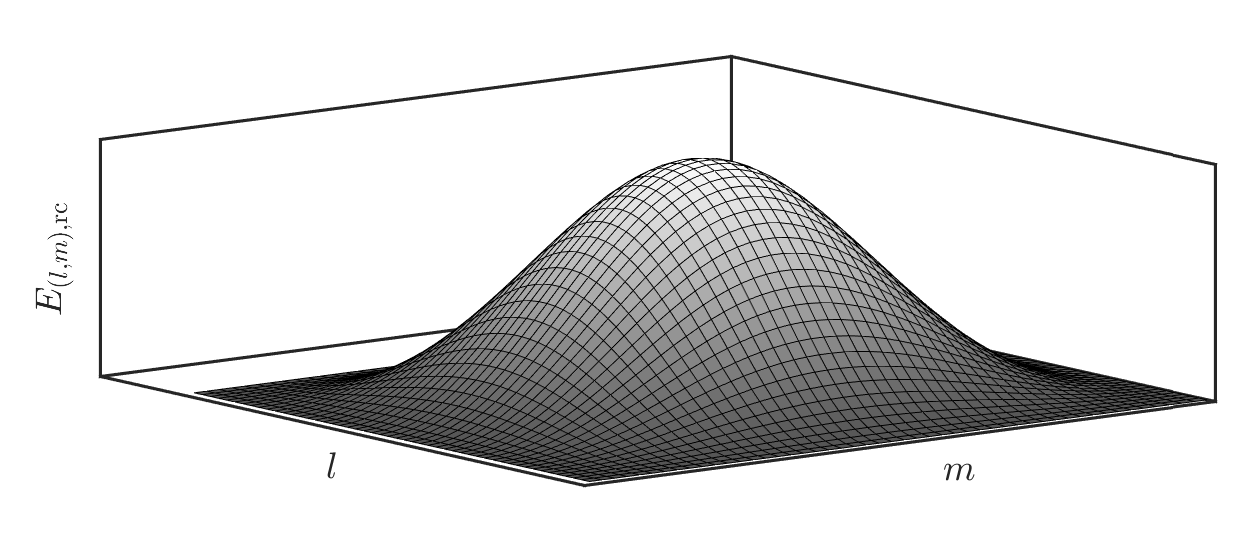
\includegraphics[width=\figWidth\textwidth]{figures/exciters/physInsp/2dHann.eps}
    \caption{A 2D raised cosine created using Eq. \eqref{eq:2DdiscRaisedCos}.\label{fig:2DHann}}
\end{figure}

\noindent
\begin{minipage}{\textwidth}
\setlstMAT
\begin{lstlisting}[caption={A \texttt{MATLAB} implementation of a 2D raised cosine.}, label=alg:2DraisedCos]
% Assuming Dirichlet boundary conditions and having initialised the following
% - center locations for the x and y-directions: l0 and m0
% - radius of the excitation r (in grid points)

ls = l0 - floor(r/2); % start location x-direction
le = l0 + floor(r/2); % end location x-direction
ms = m0 - floor(r/2); % start location y-direction
me = m0 + floor(r/2); % end location x-direction

% Create excitation matrix
e = zeros(Ny-1, Nx-1);

% Add one to hann function as the width is given in `grid spacings'
% and affects r+1 grid points
e(ms:me, ls:le) = hann(r+1) * hann(r+1)';

% Applying excitation to stacked matrix form as in Section %*\refMatlab[sec:2DwaveImplementation]*)
u = reshape(e, (Nx-1) * (Ny-1), 1);
\end{lstlisting} 
\end{minipage}
    
\section{Time-varying excitations}\label{sec:timeVaryingExcitations}
Although various types of excitation can already be modelled using the initial conditions presented in the previous section, they are temporally rigid. In other words, the time of excitation is fixed to be at the start of the simulation. In order to excite the system while the simulation is running, one can create excitations that -- on top of being spatially distributed -- have a temporal profile as well.

For the following, consider the ideal string of length $L$ (in m), where its transverse displacement is described by $u = u(x,t)$ (in m). The system is defined for $t\geq 0$ and $x\in\D$ with domain $\D = [0, L]$. The PDE of the ideal string with a time varying external force $f(t)$ (in N) is defined as (Eq. \eqref{eq:1DwavePDE})
\begin{equation}\label{eq:timeVaryingExcitation1DWave}
    \rho A\ptt u = T \pxx u + e(x)f(t)
\end{equation}
where $e(x)$ is a spatial distribution function such as those presented in Section \ref{sec:initConditionsPhysInsp} (in m$^{-1}$).

In discrete time, Eq. \eqref{eq:timeVaryingExcitation1DWave} becomes
\begin{equation}
    \rho A \dtt \uln = T \dxx \uln + E_lf^n
\end{equation}
with discrete spatial distribution $E_l$ and discrete time-varying external force $f^n$.

\subsection{Raised cosine}\label{sec:timeVaryingRaisedCos}
To yield a smooth excitation over time, one can, similar to the spatially distributed raised cosine in Eq. \ref{sec:raisedCosine}, define a temporally distributed raised cosine. Using the time of excitation $t_0\geq 0$ and excitation duration $t_\text{d}>0$ (both in s), the temporal raised cosine can be used as a force function, as
\begin{equation}\label{eq:raisedCosTemp}
    f(t) = 
    \begin{cases}
        \frac{f_\text{amp}}{2} \left(1 - \cos\left(\frac{q\pi (t - t_0)}{t_\text{d}}\right)\right), & t_\stxt \leq t \leq t_0 + t_\text{d}\\
        0, &\text{otherwise}.
    \end{cases}
\end{equation} 
As done in \cite{Webb2015, Bilbao2019}, $q$ alters the excitation to be a pluck when $q=1$ and a strike when $q=2$. Finally, $f_\text{amp}$ is the maximum force (in N). 
\def\figWidth{0.8}
\begin{figure}[t]
    \centering
    \subfloat[Pluck ($q=1$).\label{fig:timeVaryingRaisedCosPluck}]{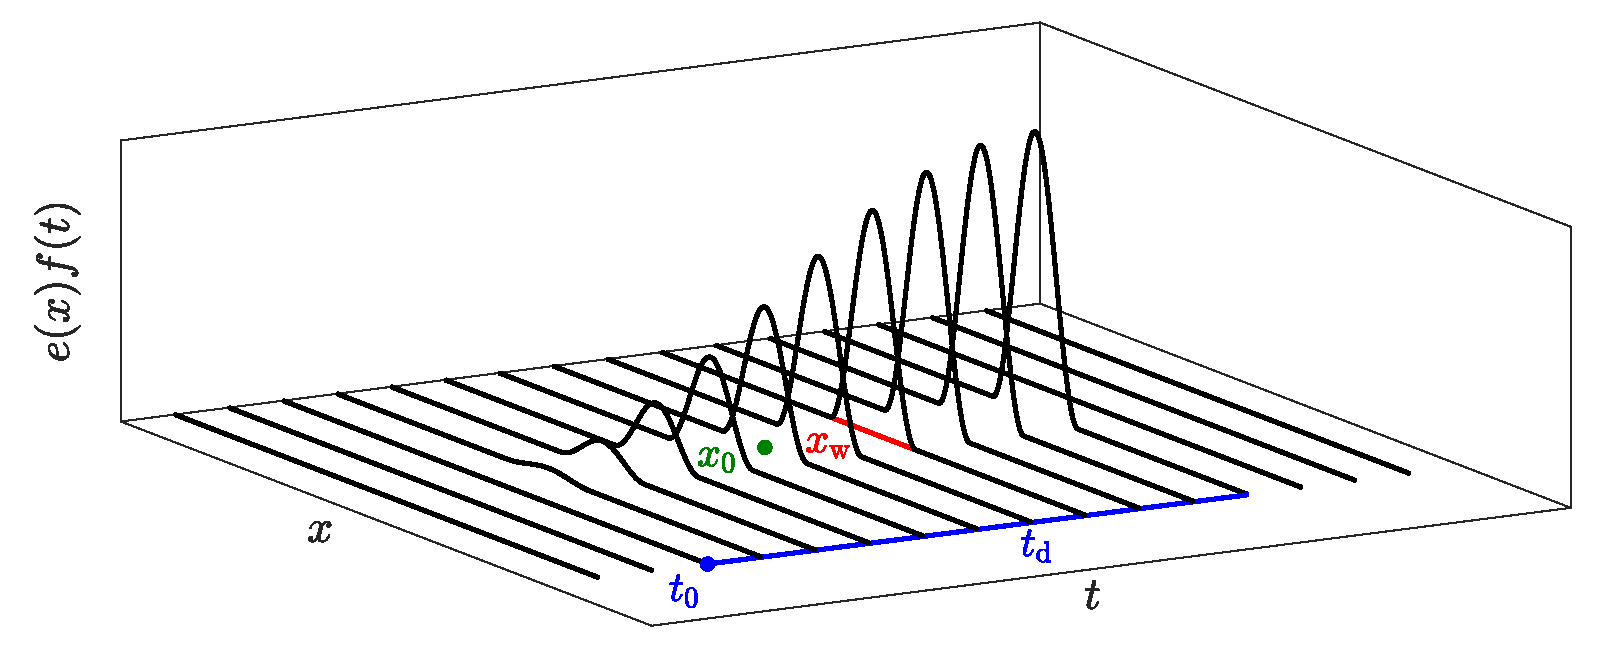
\includegraphics[width=\figWidth\textwidth]{figures/exciters/physInsp/timeVaryingRaisedCos.eps}}\\
    \subfloat[Strike ($q=2$).\label{fig:timeVaryingRaisedCosStrike}]{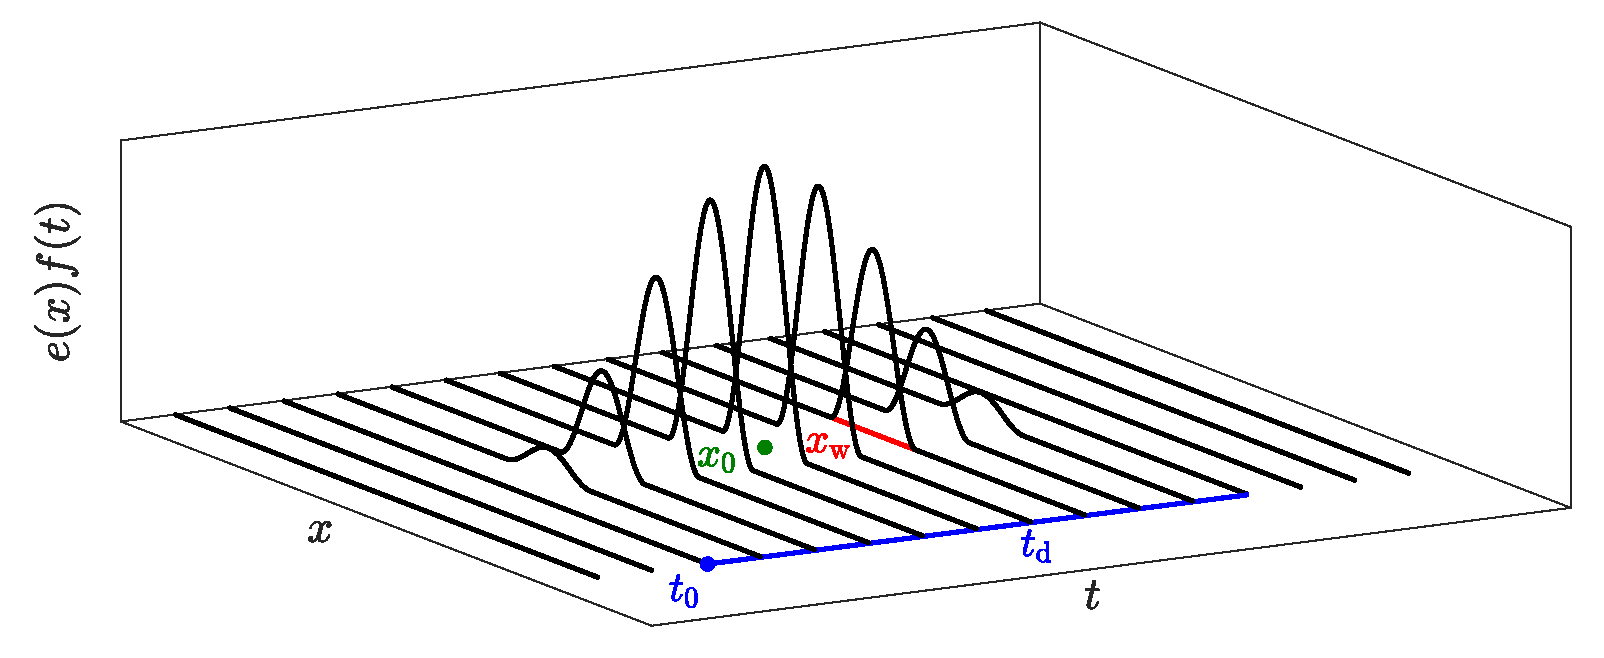
\includegraphics[width=\figWidth\textwidth]{figures/exciters/physInsp/timeVaryingRaisedCosHammer.eps}}\hfill
    \caption{The time-varying raised cosine showing a (a) pluck and a (b) strike. The location of excitation $x_0$ is shown in green, the width $x_\text{w}$ in red and the excitation start $t_0$ and duration $t_\text{d}$ in blue.\label{fig:timeVaryingRaisedCos}}
\end{figure}

As done in papers \citeP[A] and \citeP[B], the force function can be used in conjunction with the distribution functions shown in Section \ref{sec:initConditionsPhysInsp}. When used to scale a spatially distributed raised cosine as in Eq. \eqref{eq:raisedCosCont}, one can model a pluck or a strike, by setting $q=1$ or $q=2$ respectively. These alternatives are visualised in Figure \ref{fig:timeVaryingRaisedCos}. Note, that if one would like $f_\text{amp}$ to be the maximum force, one must set $e_\text{amp} = 1$ in Eq. \eqref{eq:raisedCosCont}. 

In discrete time, the force function in Eq. \eqref{eq:raisedCosTemp} becomes
\begin{equation}\label{eq:discExcitation}
    f^n = 
    \begin{cases}
        \frac{f_\text{amp}}{2}\left(1-\cos\left(\frac{q\pi (n - n_0)}{n_\text{d}}\right)\right), & n_0 \leq n \leq n_0+n_\text{d},\\
        0, &\text{otherwise}.
    \end{cases}
\end{equation}
where $n_\text{d} = \floor[t_\text{d}/k]$ is the duration of the excitation in samples.

\subsection{Pulse train}\label{sec:pulseTrain}
As already briefly introduced in Section \ref{sec:webstersExcitation}, one can create a pulse train to excite an acoustic tube. This is inspired by \cite{theBible} where the signal represents the opening and closing of the glottis. As the characteristics of the lip reed are similar to the vocal folds \cite{Richards2003}, the pulse train has been used as a test signal here (also see Section \ref{sec:lipreedTube}). A more complete model of the lip reed can be found in Chapter \ref{ch:lipreed}.

The pulse train can be created using a clipped sinusoid, which can be used as the input velocity to an acoustic tube. Algorithm \ref{alg:pulseTrain} shows an example of how to generate a pulse train. The frequency as well as the duty cycle (how much of the signal is non-zero) can be set. Figure \ref{fig:pulseTrain} shows the output of the algorithm.
\\
\\
\noindent
\begin{minipage}{\textwidth}
\setlstMAT
\begin{lstlisting}[caption={\texttt{MATLAB} code to generate a pulse train.}, label=alg:pulseTrain]
%% Pulse train generator

fs = 44100;             % Sample rate [Hz]
lengthSound = fs;       % Length of the sound [samples]
f = 440;                % Pulse train frequency
dutyC = 0.75;           % Duty cycle [0-1]
amp = 1;                % Amplitude

%% Create input signal
for n = 0:lengthSound
    if mod(n, fs / f) <= fs / f * dutyC
        vIn(n+1) = amp * sin(f * pi / dutyC * mod(n, fs / f) / fs);
    else
        vIn(n+1) = 0;
    end
end
\end{lstlisting}
\end{minipage}

% For a pulse train with a maximum amplitude of 1 and a frequency $f$ (in Hz), the following is proposed
% \def\depth{c_\text{d}}
% \begin{equation}\label{eq:pulseTrain}
%     v_\text{in} = \left[\frac{\sin(2\pi f t) - (1-2\depth)}{2\depth}\right]_+,
% \end{equation}
% where $0< \depth \leq 0.5$ is the clipping depth, and determines the duty cycle, i.e. the distance between the pulses. Finally, the $[\cdot]_+$ operator specifies `the positive part of' and is used for clipping (see Chapter \ref{ch:collisions}). 
\begin{figure}[t]
    \centering
    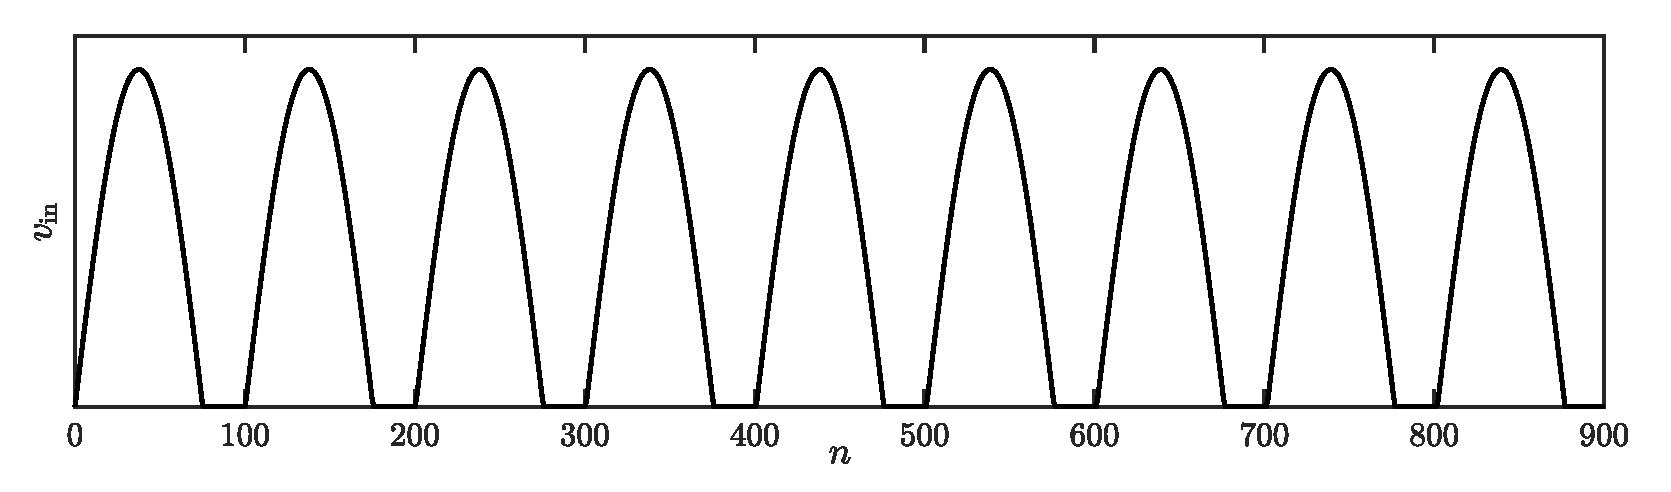
\includegraphics[width=\textwidth]{figures/exciters/physInsp/pulseTrain.eps}
    \caption{The pulse train generated using Algorithm \ref{alg:pulseTrain} ($f = 440$ Hz, duty cycle $ = 75\%$).
    \label{fig:pulseTrain}}
\end{figure}